%%%%%%%%%%%%%%%%%%%%%%%%%%%%%%%%%%%%%%%%%%%%%%%%%%%%%%%
%                  File: OPTICAmeetings.tex           %
%                  Date: 31 July 2023                 %
%                                                     %
%     For preparing LaTeX manuscripts for submission  %
%     submission to Optica meetings and conferences   %
%                                                     %
%         (c) 2018-2022 Optica Publishing Group       %
%%%%%%%%%%%%%%%%%%%%%%%%%%%%%%%%%%%%%%%%%%%%%%%%%%%%%%%

\documentclass[letterpaper, 10pt]{article} 
%% if A4 paper needed, change letterpaper to A4

\usepackage{opticameet3} %% use version 3 for proper copyright statement

%% provide authormark
\newcommand\authormark[1]{\textsuperscript{#1}}

%% standard packages and arguments should be modified as needed
\usepackage{amsmath,amssymb}
\usepackage[colorlinks=true,bookmarks=false,citecolor=blue,urlcolor=blue]{hyperref} %pdflatex
%\usepackage[breaklinks,colorlinks=true,bookmarks=false,citecolor=blue,urlcolor=blue]{hyperref} %latex w/dvipdf

\begin{document}

\title{Crecimiento de Capital respecto a la variación de tecnología o conocimiento: Modelado con Ecuaciones Diferenciales}

\author{Author name(s)}
% \address{Author affiliation and full address}
% \email{e-mail address}
%%Uncomment the following line to override copyright year from the default current year.
%\copyrightyear{2024}



\author{Jacobo Ruiz David Mauricio,\authormark{1} ~~Ordóñez del Carpio, Jyns Arturo,\authormark{2} ~~and Gutierrez Del Águila, Matías Martin \authormark{2} }

\address{\authormark{1} \href{david.jacobo@utec.edu.pe}{david.jacobo@utec.edu.pe} ~~~~202220396\\
\authormark{2} \\
\authormark{3}
}

\email{\authormark{*}opex@optica.org} %% email address is required 


\begin{abstract}
Este paper propone investigar la relación entre el crecimiento económico y el cambio tecnológico usando ecuaciones diferenciales. Se comparan dos modelos fundamentales, el Modelo Solow-Swan y el Modelo Romer, para analizar cómo el cambio tecnológico influye  en el crecimiento económico a lo largo del tiempo, el analisis matematico se centrará en el primero. El Modelo Solow-Swan se basa en la acumulación de capital físico y tecnología exógena, sugiere que el aumento de productividad solo se explica a través de inversiones directas, crecimiento poblacional y el progreso tecnológico.\cite{Chirwa18} mientras que el Modelo Romer introduce el concepto de crecimiento endógeno, el cual sugiere que el progreso tecnológico ocurre cuando se inventan nuevos productos, y esto a su vez se debe a la investigación y desarrollo (I+D) realizados por empresarios que buscan obtener beneficios económicos \cite{Chu18}. Los objetivos principales de esta investigación son analizar el impacto del cambio tecnológico en el crecimiento económico y modelar la dinámica del crecimiento económico mediante ecuaciones diferenciales.
\end{abstract}

\section*{Keywords}
\begin{flushright}
    Ecuaciones diferenciales, Crecimiento económico, Modelo Solow-Swan, Modelo Romer, Cremiento Exogeno
\end{flushright}



\section{Marco Teorico}
  Para comprender este documento es necesario comprender los conceptos clave y los modelos fundamentales que se utilizarán como base para el análisis. A continuación, se definen de manera sencilla los conceptos y modelos clave:

\begin{enumerate}
  
  \item Crecimiento Económico: El crecimiento económico es un objetivo central en la economía y se refiere al aumento sostenido de la producción de bienes y servicios en una economía a lo largo del tiempo. Este proceso conduce a un mayor nivel de vida y desarrollo económico de una sociedad. Para entender el crecimiento económico, es crucial analizar las fuentes que lo impulsan, en particular, la acumulación de capital y el cambio tecnológico.

  \item Cambio Tecnológico: El cambio tecnológico se refiere a la mejora y avance de los métodos y procesos de producción, así como a la creación de nuevos productos y tecnologías. Este factor desempeña un papel esencial en el crecimiento económico, ya que puede aumentar la productividad, mejorar la eficiencia y fomentar la innovación en una economía.
  
  \item Modelos de Crecimiento Económico: Para analizar la relación entre el crecimiento económico y el cambio tecnológico, se utilizarán dos modelos fundamentales: el Modelo Solow-Swan y el Modelo Romer.
  
  \begin{itemize}
     
    \item Modelo Solow-Swan: Este modelo, propuesto por Robert Solow y Trevor Swan en la década de 1950, se basa en la acumulación de capital físico, el crecimiento de la fuerza laboral y el progreso tecnológico como motores del crecimiento económico. En este enfoque, la tecnología se considera exógena, lo que significa que no se modifica internamente en la economía, sino que se toma como un factor dado.
  
    \item Modelo Romer: El Modelo Romer, desarrollado por Paul Romer en la década de 1980, introduce el concepto de crecimiento endógeno. En contraste con el Modelo Solow-Swan, sugiere que el progreso tecnológico es influenciado por las acciones de las empresas que buscan obtener ganancias a través de la investigación y el desarrollo (I+D). Este modelo considera que el conocimiento y la tecnología pueden ser impulsados por políticas gubernamentales y la inversión en I+D.
  
  \end{itemize}
\end{enumerate}


\section{Main Text}

\subsection{Required Elements}
All PDF submissions must contain the following items in order to be published:

\begin{enumerate}
\item Complete title
\item Complete listing of all authors and their affiliations
\item Self-contained abstract (indexers such as Google Scholar will not index papers that do not contain abstracts)
\item Appropriate copyright statement following the abstract. By default, the copyright statement will appear as \number\year \hskip.05in The Author(s). If needed, the default statement can be suppressed by use of the \verb+{abstract*}+ environment.
\item Permission and attribution for any trademarked or copyright images. Note that images of people or images owned or trademarked by other entities (including well-known logo's or cartoon characters for example) will also require official written permission.
\item Two-page limit unless designated otherwise on conference website
\end{enumerate}

\subsection{Typographical Style}
Margins and type size will be set by the Optica \LaTeX{}
commands for title, author names and addresses, abstract,
references, captions, and so on. The \texttt{opticameet3.sty} package
references \texttt{mathptmx.sty} for Times text and math fonts.
Authors who require Computer Modern font may modify the style file
or, preferably, invoke the package \texttt{ae.sty} or similar for
optimum output with Computer Modern.

\subsection{Author Names and Affiliations}
Author names should be given in full with first initials spelled out to assist with indexing.
Affiliations should follow the format division, organization, and address---and complete postal information should be given.
Abbreviations should not be used. United States addresses should end
with ``, USA.''

\subsection{Abstract} The abstract
should be limited to no more than 35 words. It should be an
explicit summary of the paper that states the problem, the methods
used, and the major results and conclusions. If another publication author is referenced in the abstract, abbreviated information
(e.g., journal, volume number, first page, year) must be
given in the abstract itself, without a reference number. (The item referenced in the abstract should be the first
cited reference  in the body.)

\subsection{Notation}
\subsubsection{General Notation}
Notation must be
legible, clear, compact, and consistent with standard usage. In
general, acronyms should be defined at first use.


\subsubsection{Math Notation}
Equations should use standard \LaTeX{} or AMS\LaTeX{} commands (sample from Krishnan \textit{et al.} \cite{Chirwa18}).

\begin{eqnarray}
\bar\varepsilon &=& \frac{\int_0?\infty\varepsilon
\exp(-\beta\varepsilon)\,{\rm d}\varepsilon}{\int_0?\infty
\exp(-\beta\varepsilon)\,{\rm d}\varepsilon}\nonumber\\
&=& -\frac{{\rm d}}{{\rm d}\beta}\log\Biggl[\int_0?\infty\exp
(-\beta\varepsilon)\,{\rm d}\varepsilon\Biggr]=\frac1\beta=kT.
\end{eqnarray}

\section{Tables and Figures}
Figures and illustrations should be incorporated directly into the
manuscript, and the size of a figure should be commensurate with the amount
and value of the information conveyed by the figure.

\begin{figure}[htbp]
  \centering
  %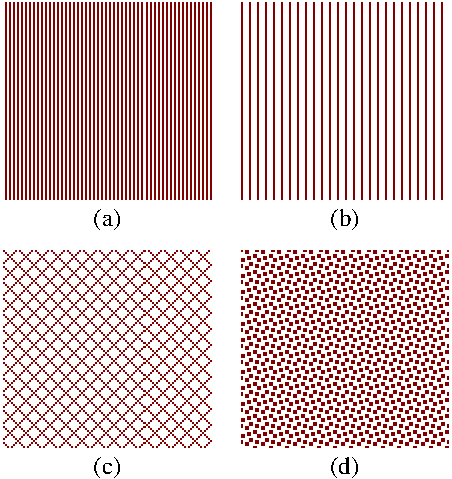
\includegraphics[width=8.3cm]{OT10000F1}
\caption{Sample figure with preferred style for labeling parts.}
\end{figure}


\begin{table}[htb]
 \centering \caption{Sample Table}
\begin{tabular}{ccc}
    \hline
    One & Two & Three \\
    \hline
    Eins & Zwei & Drei \\
    Un & Deux & Trois \\
    Jeden & Dv\v{e} & T\v{r}i \\
    \hline
   \end{tabular}
    \end{table}

No more than three figures should generally be included in the paper. Place figures as close as possible to where they
are mentioned in the text. No part of a figure should extend beyond text width, and text should not wrap around figures. Please provide permission and attribution for any trademarked or copyright images.

\section{References}
References should be cited with the \verb+\cite{}+ command.
Bracketed citation style, as opposed to superscript, is preferred
\cite{Chirwa18,Chu18,masters93,shoop97,kalman76,craig96,steup96}.
The \texttt{opticameet3.sty} style file references \texttt{cite.sty}. Comprehensive journal abbreviations are available on the Crossref web site:
\href{http://www.crossref.org/titleList/}{http://www.crossref.org/titleList/}.

\begin{thebibliography}{99} %% use BibTeX or add references manually



\bibitem{Chirwa18}Chirwa, T. G., \& Odhiambo, N. M. (2018). Exogenous and endogenous growth models: A critical review. Comparative Economic Research. Central and Eastern Europe, 21(4), 63-84.\\
\url{https://www.econstor.eu/handle/10419/259181}.

\bibitem{Chu18}Chu, A. C. (2018). From Solow to Romer: Teaching endogenous technological change in undergraduate economics. International Review of Economics Education, 27, 10-15.


\bibitem{masters93} T. Masters, \emph{Practical Neural Network Recipes in C++} (Academic, 1993).

\bibitem{shoop97} B. L. Shoop, A. H. Sayles, and D. M. Litynski, ``New devices for optoelectronics: smart pixels,''
in \emph{Handbook of Fiber Optic Data Communications},
C. DeCusatis, D. Clement, E. Maass, and R. Lasky, eds. (Academic, 1997), pp. 705--758.

\bibitem{kalman76} R. E. Kalman,``Algebraic aspects of the generalized inverse of a rectangular matrix,'' in
\emph{Proceedings of Advanced Seminar on Generalized Inverse and Applications}, M. Z. Nashed, ed. (Academic, 1976), pp. 111--124.

\bibitem{craig96} R. Craig and B. Gignac, ``High-power 980-nm pump lasers,''
in \emph{Optical Fiber Communication Conference}, Vol. 2 of 1996 OSA Technical Digest Series (Optical Society of America, 1996), paper ThG1.

\bibitem{steup96} D. Steup and J. Weinzierl, ``Resonant THz-meshes,''
presented at the Fourth International Workshop on THz Electronics, Erlangen-Tennenlohe, Germany, 5--6 Sept. 1996.

\end{thebibliography}

\end{document}
